\chapter{Landasan Teori}
\label{chap:definition}

\section{\textsl{Data Mining}}

\textsl{Data mining} merupakan merupakan proses yang melakukan pengambilan inti sari atau penggalian \textsl{knowledge} dari data yang besar dan merupakan salah satu langkah dari \textsl{knowledge discovery}.


\begin{figure}[H]
\centering
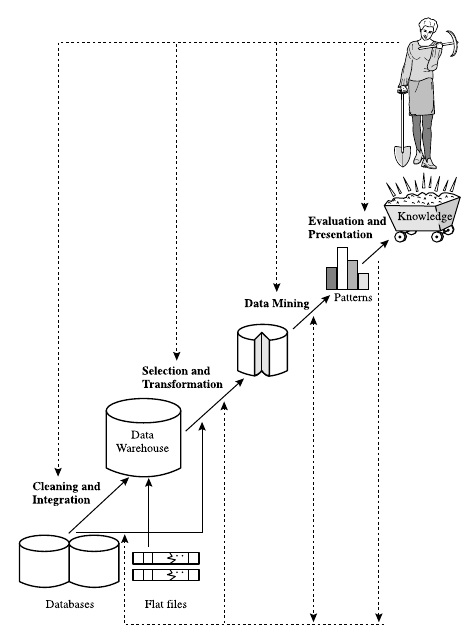
\includegraphics[scale=0.9]{Gambar/tahapdatamining.jpg}
\caption[Tahap \textsl{Data Mining}]{Tahap \textsl{Data Mining}, Diterjemahkan dari \cite{DM}} 
\label{fig:tahapDataMining}
\end{figure}

Menurut \cite{DM}, \textsl{knowledge discovery} dapat dibagi menjadi 7 tahap (gambar \ref{fig:tahapDataMining}):
\begin{enumerate}
	\item \textsl{Data cleaning}
	\item \textsl{Data integration}
	\item \textsl{Data selection}
	\item \textsl{Data transformation}
	\item \textsl {Data mining}
	\item \textsl{Pattern Evaluation}
	\item \textsl{Knowledge presentation}
\end{enumerate}


Tahap pertama hingga keempat merupakan bagian dari \textsl{data preprocessing}, dimana data-data disiapkan untuk dilakukan penggalian data. Tahap \textsl{data mining} merupakan tahap dimana melakukan penggalian data. Tahap keenam merupakan tahap pencarian pola yang merepresentasikan \textsl{knowledge}. Sedangkan tahap terakhir merupakan visualisasi dan representasi dari \textsl{knowledge} yang sudah diperoleh dari tahap sebelumnya.


\subsection{\textsl{Data Cleaning}}
\textsl{Data cleaning} merupakan tahap \textsl{data mining} untuk menghilangkan \textsl{missing value} dan \textsl{noisy data}. Pada umumnya, \textsl{data} yang diperoleh dari \textsl{database} terdapat nilai yang tidak sempurna seperti nilai yang hilang, nilai yang tidak valid atau salah ketik. Atribut dari suatu \textsl{database} yang tidak relevan atau redudansi bisa diatasi dengan menghapus atribut atau record tersebut. Contoh studi data yang memiliki \textsl{missing value} dan \textsl{noisy data} dapat dilihat pada table \ref{table:contohMissingNNoisy}

\begin{table}[h]
\centering
\caption{table mengandung \textsl{missing value} dan \textsl{noisy data}}
\label{table:contohMissingNNoisy}
\begin{tabular}{|l|l|l|l|l|}
\hline
IdPenjualan & NamaBarang & Customer & Harga  & BanyakBarang \\ \hline
1           & Mouse      & Elvin    & 45000  & 2            \\ \hline
2           & Keyboard   & Alleria  & -35000 & 1            \\ \hline
3           & Monitor    &          & 225000 & 1            \\ \hline
\end{tabular}
\end{table}

Dapat dilihat, pada idPenjualan 2, harga dari keyboard adalah -35000, itu merupakan \textsl{noisy data} karena tidak mungkin nilai harga suatu barang dibawah 0. Pada idPenjualan 3, kolom \textsl{customer} tidak memiliki nilai, dan itu merupakan \textsl{missing value}.

\subsubsection{\textsl{Missing Values}}
\textsl{Missing values} akan mengganggu proses \textsl{data mining} pada komputer dan dapat menghasilkan nilai akhir yang tidak sesuai. Terdapat beberapa teknik untuk mengatasi \textsl{missing values} yaitu
	\begin{itemize}
		\item Membuang tuple yang mengandung nilai yang hilang\textit{\textit{}}
		\item Mengisi nilai yang hilang secara manual
		\item Mengisi nilai yang hilang dengan menggunakan nilai konstan yang bersifat umum
		\item Menggunakan nilai rata-rata dari suatu atribut untuk mengisi nilai yang hilang
	\end{itemize}
\subsubsection{\textsl{Noisy Data}}
\textsl{Noisy data} merupakan nilai yang berasal dari error atau tidak valid. \textsl{Noisy data} dapat dihilangkan dengan menggunakan teknik \textsl{smoothing}. Terdapat 3 metode untuk menghilangkan \textsl{noisy data} yaitu
	\label{teknikBinning}
	\begin{itemize}
		\item \textsl{Binning}, merupakan metode pengisian data sesuai dengan proses yang dilakukan pada data tersebut
		\item \textsl{Regression}, merupakan metode yang mencari detail persamaan atribut untuk memprediksikan suatu nilai
		\item	\textsl{Clustering}, merupakan metode pengelompokan dimana ditemukan \textsl{outliers} yang dapat dibuang. Outliers merupakan data yang berada diluar kelompok yang sesuai dengan observasi atau penelitian.
	\end{itemize}

%\subsubsection{\textsl{Data Cleaning as a Process}}
%Tahap pertama pada \textsl{data cleaning} adalah \textsl{discrepancy detection}. Ketidakcocokan dapat dikarenakan oleh beberapa faktor, termasuk desain data yang buruk, kesalahan manusia ketika memasukan data, dan data yang sudah kadarluarsa. Ketidakcocokan ini juga dapat disebabkan tidak konsisten representasi data dan kode atau dikarenakan kesalahan perangkat ketika melakukan pemasukan data.

%Untuk mempermudah pencarian ketidakcocokan tersebut, kita dapat membuat sebuah data yang berisi informasi mengenai data atau biasa disebut \textsl{metadata}. Pada tahap ini, penulisan \textsl{script} bisa ditulis dengan cara masing-masing. Disini, dapat ditemukan \textsl{noise}, \textsl{outliers}, dan nilai-nilai yang tidak cocok atau tidak konsisten.

%Data juga harus diperiksa dengan \textsl{unique rules}, \textsl{consecutive rules}, dan \textsl{null rules}. \textsl{unique rules} mengatakan bahwa setiap nilai dari sebuah atribut harus berbeda dengan nilai yang lain pada atribut tersebut. \textsl{Consecutive rules} mengatakan bahwa tidak boleh ada nilai yang hilang diantara nilai tertinggi dan terendah untuk sebuah atribut, dan semua nilai harus bersifat unik. \textsl{null rules} menspesifikasikan penggunaan nilai \textsl{blanks} atau kosong, tanda tanya, karakter spesial, atau \textsl{string} yang dapat menandakan bahwa nilai tersebut bersifat kosong.

%Tahap deteksi ketidakcocokan ini dapat dibantu juga dengan menggunakan \textbf{data scrubbing tools} dan \textbf{data auditing tools}. \textbf{data scrubbing tools} akan menggunakan sebuah domain data untuk melakukan pencarian ketidakcocokan data dan membetulkan data tersebut dengan menggunakan teknik \textsl{parsing} dan \textsl{fuzzy matching}. \textbf{Data auditing tools} akan mencari ketidakcocokan dengan melakukan analisa data untuk menemukan \textsl{rules}, relasi, dan mendeteksi data yang melanggar hal tersebut.

%Beberapa data dapat diperbaiki dengan cara manual, namun sebagian besar data akan membutuhkan \textsl{data transformation} untuk membetulkan data tersebut.

\subsection{\textsl{Data Integration}}
\textsl{Data integration} merupakan tahap menggabungkan data dari berbagai sumber. Sumber tersebut bisa termasuk beberapa \textsl{database}, \textsl{data cubes}, atau bahkan \textsl{flat data}. \textsl{Data cube} merupakan teknik pengambilan data-data dari \textsl{data warehouse} dan dilakukan operasi agregasi sesuai dengan kondisi tertentu (contoh, penjumlahan total penjualan per tahun dari 2005-2010). Sedangkan \textsl{flat data} merupakan data yang disimpan dengan cara apapun untuk merepresentasikan database model pada sebuah data baik berbentuk \textsl{plain text file} maupun \textsl{binary file}. 

Tahap ini harus dilakukan secara teliti terutama ketika dalam memasangkan nilai-nilai yang berasal dari sumber yang berbeda. Pada tahap ini, perlu dilakukan identifikasi data apakah data tertentu harus dimasukkan atau tidak agar data yang diperoleh tidak terlalu besar. \textsl{Data integration} yang baik merupakan integrasi yang dapat memaksimalkan kecepatan dan meningkatkan akurasi dari proses \textsl{data mining}. Contoh studi kasus dari \textsl{data integration}, jika suatu perusahaan sepatu A memiliki dua pabrik dengan \textsl{database} lokal pada masing-masing pabrik, jika akan dilakukan \textsl{data mining} pada kedua \textsl{database }tersebut, maka kedua \textsl{database} akan digabung dan perlu diperhatikan serta diperbaiki nilai-nilai seperti \textsl{primary key}, atribut, dan lain-lain agar tidak terjadi \textsl{error} pada \textsl{database} yang sudah digabung. Proses dari penggabungan hingga perbaikan nilai-nilai pada kedua database tersebut adalah proses \textsl{data integration}.

\subsection{\textsl{Data Selection}}
Proses dimana data-data yang relevan dengan analisis akan diambil dari database dan data yang tidak relevan akan dibuang. Sebagai contoh kasus, jika akan dilakukan analisa mengenai nilai mahasiswa pada table nilai yang memiliki atribut sebagai berikut:
	\begin{itemize}
		\item NPMMahasiswa
		\item NamaMahasiswa
		\item JenisKelamin
		\item Alamat
		\item MataKuliah
		\item NilaiART
		\item NilaiUTS
		\item NilaiUAS
	\end{itemize}
Maka, atribut yang berpotensi diambil adalah MataKuliah, NilaiART, NilaiUTS, NilaiUAS, sedangkan atribut yang akan dibuang adalah NPMMahasiswa, NamaMahasiswa JenisKelamin, dan Alamat karena tidak terlalu berhubungan dengan analisa.

\subsection{\textsl{Data Transformation}}
\textsl{Data transformation} merupakan tahap pengubahan data agar siap dilakukan proses \textsl{data mining}. \textsl{Data transformation} bisa melibatkan:
	\begin{itemize}
		\item \textsl{Smoothing}, proses untuk membuang \textsl{noise} seperti yang dilakukan pada tahap \textsl{data cleaning}
		\item \textsl{Aggregation}, proses mengganti nilai-nilai menjadi suatu nilai yang dapat mewakili nilai sebelumnya
		\item \textsl{Generalization}, proses dimana membuat suatu nilai yang bersifat khusus menjadi nilai yang bersifat umum
		\item \textsl{Normalization}, proses dimana suatu nilai dapat diubah skalanya menjadi nilai yang lebih kecil dan spesifik
		\item \textsl{Attribute construction}, proses membuat atribut baru yang berasal dari beberapa atribut untuk membantu proses data mining
	\end{itemize}
	
\subsubsection{\textsl{Smoothing}}
\textsl{Smoothing} merupakan bagian dari \textsl{data cleaning} untuk menghilangkan \textsl{noise} pada database. Teknik dari \textsl{smoothing} adalah \textsl{binning}, \textsl{regression}, dan \textsl{clustering}. Penjelasan teknik \textsl{smoothing} dapat dilihat pada \ref{teknikBinning}, bagian \textsl{noisy data}.

\subsubsection{\textsl{Aggregation}}
\textsl{Aggregation}, dimana suatu kesimpulan atau hasil dari \textsl{aggregation operation} yang disimpan dalam database. Contoh studi kasus, jika terdapat suatu database dari toko A, kita dapat menggunakan operasi \textsl{aggregation} untuk mencari total pendapatan dengan rentang hari tertentu.

\subsubsection{\textsl{Generalization}}	
\textsl{generalization}, dimana suatu data yang memiliki nilai \textsl{primitive} atau \textsl{low level} diubah menjadi \textsl{high level} dengan menggunakan konsep hirarki. Contoh studi kasus, nilai pada atribut umur dapat dikelompokkan menjadi muda, dewasa, tua.	
	
\subsubsection{\textsl{Normalization}}
Atribut dapat dinormalisasi dengan memberi skala pada nilainya sehingga nilai tersebut menjadi suatu range yang lebih spesifik dan kecil seperti 0,0 sampai 1,0.
Terdapat beberapa teknik normalisasi, dua diantaranya yaitu, \textsl{min-max normalization} dan \textsl{z-score normalization}. \textsl{Min-max normalization} akan mengubah semua nilai menjadi nilai dengan skala tertentu. Dengan menggunakan rumus 

\begin{displaymath}
	\nu' = \frac{\nu-min_{A}}{max_{A}-min_{A}}(newMax_{A}-newMin_{A})+newMin_{A}	
\end{displaymath}

Contoh kasus, misalkan nilai minimun dan maximum dari suatu pendapatan adalah 12.000 dan 98.000, akan diubah menjadi berskala antara 0,0 sampai 1,0. Jika ada nilai pendapat yang baru, yaitu 73.600, maka akan menjadi

\begin{displaymath}
\frac{73.600-12.000}{98.000-12.000} (1,0-0)+0 = 0,716
\end{displaymath}

\textsl{z-score normalization} merupakan normalisasi berdasarkan nilai rata-rata dan standar deviasi dari nilai-nilai atribut dengan cara

\begin{displaymath}
\nu' = \frac{\nu-\overline{A}}{\sigma_{A}}
\end{displaymath}

Contoh kasus, misal nilai rata-rata dan standar deviasi dari nilai-nilai atribut pendapatan adalah 54.000 dan 16.000. Dengan \textsl{z-score}, jika ada nilai pendapatan baru yaitu 73600, maka akan diubah menjadi

\begin{displaymath}
\frac{73.600-54.000}{16.000} = 1,225 
\end{displaymath}

\subsubsection{\textsl{Attribute Construction}}
\textsl{Attribute Construction} merupakan teknik menambahkan atribut baru yang berdasarkan dari atribut yang sudah ada guna menambah akurasi. Contoh kasus, dibuat atribut baru bernama area berdasarkan atribut panjang dan lebar. 

%\subsubsection{\textsl{Data Reduction}}
%Proses \textsl{aggregation} dan \textsl{generalization} akan dilakukan dalam bentuk proses \textsl{data reduction} dan \textsl{Data Cube Aggregation}.
%\textsl{Data reduction} dan dilakukan untuk mendapatkan nilai yang representif namun tetap menjaga keakuratan hasil \textsl{data mining}. Terdapat beberapa cara dalam mengimplementasikan \textsl{data reduction} yaitu
%	\begin{itemize}
%		\item \textsl{Data subset selection}
%		\item \textsl{Dimensionality reduction}
%		\item \textsl{Numerosity reduction}
%		\item \textsl{Discretization and concept hierarchy generation}
%	\end{itemize}	

%\subsubsection {\textsl{Attribute Subset Selection}}
%\textsl{Attribute subset selection} merupakan salah satu cara melakukan \textsl{data reduction} dengan menghilangkan atribut-atribut yang tidak relevan atau data yang redudansi. Hal ini dapat mempermudah pencarian pola dikarenakan atribut yang tidak relevan tidak ada. Tujuan dari \textsl{attribute subset selection} adalah memperoleh set data yang paling sedikit yang tetap menghasilkan probabilitas penyebaran data kelas tetap mirip dengan set data sebelum dikurangi atributnya. 
%Contoh studi kasus, jika toko CD ingin mencari apakah para konsumen tertarik dan membeli CD baru, maka atribut nama dan nomor telepon dari data konsumen tidak terlalu relevan dengan tujuan \textsl{mining} pada kasus ini, sedangkan jenis\_kelamin dan musik\_kesukaan dari konsumen bisa menjadi atribut yang relevan. 

%\subsubsection {\textsl{Dimensionality Reduction}}
%\textsl{Dimensionality Reduction} merupakan metode pengurangan nilai secara acak dengan cara melakukan konversi data. Jika data original dapat dibuat ulang dari data yang sudah dikompresi tanpa kehilangan informasi, maka akan dikatakan \textsl{lossless}, namun jika hanya mendapatkan data pendekatannya saja, akan disebut lossly \cite{DM}.

%\subsubsection {\textsl{Numerosity Reduction}}
%\textsl{Numerosity Reduction} merupakan metode dimana data diganti atau ditentukan dengan cara parametik atau nonparametrik.

%\subsubsection {\textsl{Discretization and Concept Hierarchy Generation}}
%lewat dulu

\subsection{\textsl{Data Mining}}

Pada tahap ini, akan dilakukan proses \textsl{data mining} dengan menggunakan input data yang sudah diproses pada tahap sebelumnya (\textsl{data cleaning, data selection, data integration,} dan /\textsl{data transformation}).

\subsubsection{\textsl{Classification and Prediction}}
\textsl{Classification} merupakan pemodelan yang dibangun untuk memprediksikan label kategori, seperti "baik", "cukup", dan "buruk" dalam sistem penilaian sikap seorang siswa atau "mini bus", "bus", atau "sedan" dalam kategori tipe mobil. Kategori tersebut dapat direpresentasikan dengan menggunakan nilai diskret. Nilai diskret merupakan nilai yang terpisah dan berbeda, seperti 1 atau 5. Kategori yang direpresentasikan oleh nilai diskret maka akan menjadi nilai yang terurut dan tidak memiliki arti, seperti 1,2,3 untuk merepresentasikan kategori tipe mobil "mini bus", "bus", dan "sedan".

\textsl{Prediction} merupakan model yang dibangun untuk meramalkan fungsi nilai kontinu atau \textsl{ordered value}. \textsl{Ordered value} merupakan nilai yang terurut dan berlanjut. Contoh studi kasus untuk pemodelan prediction adalah seorang marketing ingin meramalkan seberapa banyak konsumen yang akan belanja di sebuah toko dalam waktu satu bulan. Pemodelan tersebut disebut \textsl{predictor}. \textsl{Regression Analysis}, merupakan metodologi statistik yang digunakan untuk \textsl{numeric prediction}. \textsl{Classification} dan \textsl{numeric prediction} merupakan dua jenis utama dalam masalah prediksi.

\textsl{Data Classification} merupakan proses untuk melakukan klasifikasi. \textsl{Data classification} memiliki dua tahap proses, yaitu \textsl{learning step} dan tahap klasifikasi seperti pada ilustrasi di gambar \ref{fig:tahapDataClassification}. \textsl{Learning step} merupakan langkah pembelajaran, di mana algoritma klasifikasi membangun \textsl{classification rules} (yang berisi syarat atau aturan sebuah nilai masuk ke dalam kategori tertentu) dengan cara menganalisis \textsl{training set} yang merupakan \textsl{database tuple}. Karena pembuatan \textsl{classification rules} menggunakan \textsl{training set}, yang dikenal juga sebagai \textsl{supervised learning}. 
Pada tahap kedua, dilakukan proses klasifikasi nilai berdasarkan \textsl{classification rules} yang sudah dibangun dari tahap pertama.

\begin{figure}
\centering
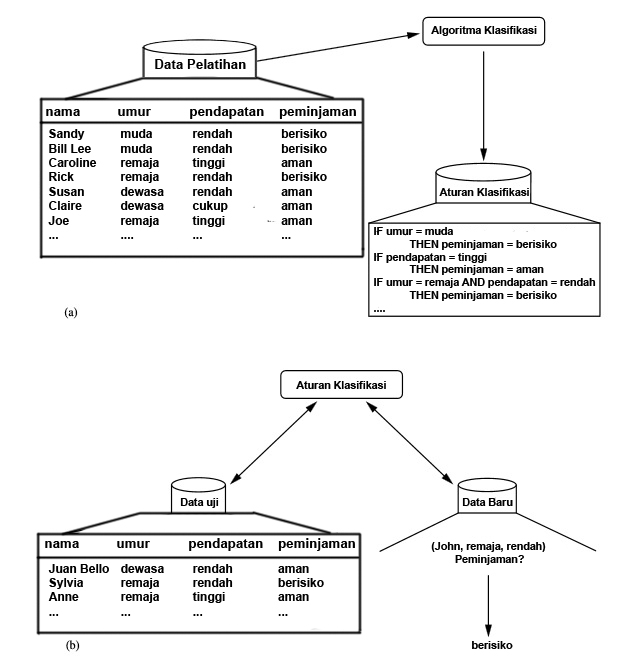
\includegraphics[scale=0.8]{Gambar/tahapdataclassification.jpg}
\caption[Tahap \textsl{data classification}]{Tahap \textsl{data classification}, Diterjemahkan dari \cite{DM}} 
\label{fig:tahapDataClassification}
\end{figure}

\subsubsection{\textsl{Decision Tree}}
Salah satu cara pembuatan \textsl{classification rules} pada \textsl{Data Classification} adalah dengan membuat \textsl{decision tree} (pohon keputusan). \textsl{Decision tree} merupakan \textsl{flowchart} yang berbentuk pohon, dimana setiap node internal (\textsl{nonleaf} node) merupakan hasil test dari atribut, setiap cabang merepresentasikan output dari test, dan setiap node daun memiliki \textsl{class label}. Bagian paling atas dari pohon disebut \textsl{root node}. Contoh studi kasus, pohon keputusan untuk menentukan apakah seorang konsumen akan membeli komputer atau tidak (ilustrasi pohon keputusan pada gambar \ref{fig:decisionTree}) 

\begin{figure}
\centering
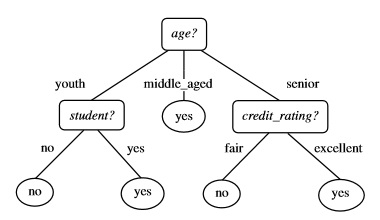
\includegraphics[scale=1]{Gambar/decisiontree.jpg}
\caption[Contoh \textsl{decision tree}]{Contoh \textsl{decision tree}, Diterjemahkan dari \cite{DM}} 
\label{fig:decisionTree}
\end{figure}

\paragraph{\textsl{Decision Tree Induction}}

\textsl{Decision tree induction} merupakan pelatihan pohon keputusan dari tupel pelatihan kelas berlabel. Terdapat beberapa teknik untuk membuat \textsl{decission tree} dua diantaranya adalah ID3 dan C4.5. ID3 merupakan teknik pembuatan \textsl{decision tree} dengan memanfaatkan \textsl{entropy} dan \textsl{gain info} untuk menentukan atribut yang terbaik untuk node pada \textsl{decision tree}. Sedangkan C4.5 merupakan teknik lanjutan dari ID3 yang menggunakan \textsl{gain ratio} untuk melakukan pengecekan pada nilai \textsl{gain info}. Kedua teknik tersebut menggunakan pendekatan \textsl{greedy} yang merupakan \textsl{decission tree} yang dibangun secara \textsl{top-down recursive divide and conquer}. Algoritma yang diperlukan secara umum sama, hanya berbeda pada \textsl{attribute\_selection\_method}. Berikut algoritma untuk membuat pohon keputusan dari suatu tupel pelatihan.


\begin{algorithmic}[1]
	\REQUIRE Partisi data, D, merupakan set data pelatihan dan kelas label
	\REQUIRE \textsl{attribute\_list}, merupakan set dari atribut kandidat
	\REQUIRE \textsl{Attribute\_selection\_method}, prosedur untuk menentukan \textsl{splitting criterion}. Pada input ini, terdapat juga data \textsl{splitting\_attribute} dan mungkin salah satu dari \textsl{split point} atau \textsl{splitting subset}
	\ENSURE Pohon keputusan
	\STATE Membuat node N;
	\IF{tuple pada D merupakan kelas yang sama, C} 
	  \RETURN N sebagai node daun dengan label kelas C;
	\ENDIF
	\IF{attribute\_list tidak ada nilai atau kosong}
		\RETURN N sebagai node daun dengan label kelas yang terpaling banyak pada D; \COMMENT {majority voting}
	\ENDIF
	\STATE memanggil method Attribute\_selection\_method(D, atribute\_list) untuk mencari nilai terbaik splitting\_criterion;
	\STATE menamakan node N dengan splitting\_criterion;
	\IF{splitting\_attribute merupakan nilai discrete and multiway splits diizinkan}
		\STATE attribute\_list $\leftarrow$ attribute\_list - splitting\_attribute; \COMMENT{menghapus splitting\_attribute}
	\ENDIF
	\FORALL{hasil j dari splitting\_criterion}
		\STATE D\lowercase{j} merupakan himpunan data tupel D yang sesuai dengan j;
		\IF{D\lowercase{j} tidak ada nilai atau kosong}
			\STATE melampirkan daun yang diberi label dengan kelas mayoritas di D ke node N;
		\ELSE
			\STATE melampirkan node yang dikembalikan oleh generate\_decision\_tree(D\lowercase{j}, attribute\_list) ke node N;
		\ENDIF
	\ENDFOR
\RETURN N;
\end{algorithmic}

Pohon keputusan akan dimulai dengan satu node, yaitu N, merepresentasikan tuple pelatihan pada D (baris 1)

Jika tuple di D memiliki kelas yang sama semua, maka node N akan menjadi daun dan diberi label dari kelas tersebut (baris 2 sampai 4). Perlu diketahui bahwa baris 5 sampai 7 akan mengakhiri kondisi.

Jika tuple di D ada kelas yang berbeda, maka algoritma akan memanggil \textsl{attribute\_selection\_method} untuk menentukan \textsl{splitting criterion}. \textsl{Splitting criterion} akan menentukan atribut pada node N yang merupakan nilai terbaik untuk memecah nilai atribut pada tuple ke dalam kelas masing-masing. (baris 8)

Node N akan diisi dengan hasil dari \textsl{splitting criterion} (baris 9). Kemudian kriteria tersebut agak dibentuk cabangnya masing-masing sesuai pada baris 13 dan 14. Terdapat tiga kemungkinan bentuk kriteria jika A merupakan \textsl{splitting\_attribute} yang memiliki nilai unik seperti \{a$_{1}$, a$_{2}$, ..., a$_{v}$\} seperti pada gambar \ref{fig:splitPoint}, yaitu,

\begin{enumerate}
	\item \textsl{Discrete valued}: cabang yang dihasilkan memiliki kelas dengan nilai diskret. Karena kelas yang dihasilkan diskret dan hanya memiliki nilai yang sama pada cabang tersebut, maka \textsl{attribut\_list} akan dihapus (baris 10 sampai 12)
	\item \textsl{Continuous values}: cabang yang dihasilkan memiliki jarak nilai untuk memenuhi suatu kondisi (contoh: A <= split\_point), dimana nilai \textsl{split\_point} adalah nilai pembagi yang dikembalikan oleh \textsl{attribute\_selection\_method}
	\item \textsl{Dicrete valued and a binary tree}: cabang yang dihasilkan adalah dua berupa nilai iya atau tidak dari "`apakah A anggota S$_{a}$"', dimana S$_{a}$ merupakan subset dari A, yang dikembalikan oleh \textsl{Attribute\_selection\_method}
\end{enumerate}


\begin{figure}
\centering
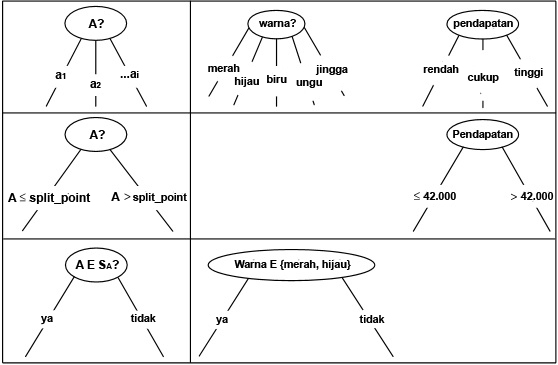
\includegraphics[scale=1]{Gambar/jenishasilsplitpoint.jpg}
\caption[Jenis-jenis \textsl{split point}]{Jenis-jenis \textsl{split point}, Diterjemahkan dari \cite{DM}} 
\label{fig:splitPoint}
\end{figure}

Kemudian, akan dipanggil kembali algoritma \textsl{decision tree} untuk setiap nilai hasil pembagian pada tuple, D$_{j}$  (baris 18).

Rekursif tersebut akan berhenti ketika salah satu dari kondisi terpenuhi, yaitu

\begin{enumerate}
	\item Semua tuple pada partisi D merupakan bagian dari kelas yang sama.
	\item Sudah tidak ada atribut yang dapat dilakukan pembagian lagi (dilakukan pengecekan pada baris 4). Disini, akan dilakukan \textsl{majority voting} (baris 6) yang akan mengkonversi node N menjadi \textsl{leaf} dan diberi label dengan kelas yang terbanyak pada D.
	\item Sudah tidak ada tuple yang dapat diberi cabang, D$_{j}$ sudah kosong (baris 15) dan \textsl{leaf} akan dibuat dengan \textsl{majority class} pada D (baris 16).
\end{enumerate}

Pada baris 21, akan dikembalikan nilai \textsl{decision tree} yang telah dibuat.

\paragraph{\textsl{Attribute Selection Measure}} merupakan suatu hirarki untuk pemilihan \textsl{splitting criterion} yang terbaik yang memisah partisi data (D), tuple pelatihan kelas label ke dalam kelas masing-masing. \textsl{Attribute Selection Measure} menyediakan peringkat untuk setiap atribut pada training tuple. Jika \textsl{splitting criterion} merupakan nilai \textsl{continous} atau \textsl{binary trees}, maka nilai \textsl{split point} dan \textsl{splitting subset} harus ditentukan sebagai bagian dari \textsl{splitting criterion}. Contoh dari \textsl{attribute selection measure} adalah \textsl{information gain}, \textsl{gain ratio}, dan \textsl{gini index}.

Notasi yang digunakan adalah sebagai berikut. D merupakan data partisi, set pelatihan dari \textsl{class-labeled} tuple. Jika label kelas atribut memiliki m nilai yang berbeda yang mendifinisikan m kelas yang berbeda, $C_{i}$ (for i=1,...,m). C$_{i,d}$ menjadi kelas tuple dari C$_{i}$ di D. |D| dan |C$_{i,d}$| merupakan banyak tuple pada D dan C$_{i,d}$.

\subsubsection{ID3}

ID3 merupakan teknik untuk membuat \textsl{decision tree} dengan menggunakan \textsl{information gain} sebagai \textsl{attribute selection measure} untuk memilih atribut. Cara ID3 mendapatkan \textsl{information gain} dengan menggunakan \textsl{entropy}. \textsl{Entropy} adalah ukuran \textsl{impurity} (ketiadaan informasi) dari suatu data. Cara mendapatkan nilai \textsl{entropy} adalah

%\textsl{Information} menurut Claude Shannon dalam \textsl{information theory} adalah ukuran \textsl{pure} dari suatu data. Suatu data yang \textsl{pure} jika data tersebut memiliki tuple dengan \textsl{class} yang sama. ID3 menggunakan \textsl{information gain} sebagai \textsl{attribute selection measure} yang melakukan pemilihan atribut berdasarkan informasi yang terkandung dalam pesan. Cara ID3 mendapatkan \textsl{information gain} dengan menggunakan \textsl{entropy}. \textsl{Entropy} adalah ukuran \textsl{impurity} dari suatu data. Cara mendapatkan nilai \textsl{entropy} adalah

\begin{displaymath}
	Info(D) = -\sum_{i=1}^{m} p_{i} \log_2(p_{i})
\end{displaymath}

Dimana $p_{i}$ merupakan probabilitas tuple pada D terhadap class C$_{i}$, dapat diperoleh dengan |C$_{i,d}$|/|D|. Info(D) merupakan nilai rata-rata \textsl{entropy} dari suatu label kelas pada tuple D. Untuk mengetahui atribut mana yang paling baik untuk dijadikan \textsl{splitting attribute}, adalah dengan cara menghitung nilai \textsl{entrophy} dari suatu atribut kemudian diselisihkan dengan nilai \textsl{entropy} dari D. Jika pada tuple D, memiliki atribut A dengan v nilai yang berbeda, maka menghitung \textsl{entropy} dari suatu atribut adalah

\begin{displaymath}
	Info_A(D) = \sum_{j=1}^v \frac{|D_j|}{|D|} \times Info(D_j)
\end{displaymath}

|D$_{j}$|/D merupakan angka yang menghitung bobot dari suatu partisi.

Setelah mendapatkan nilai Info(D) dan Info$_{A}$(D), \textsl{information gain} dapat diperoleh dari selisih nilai Info(D) dan Info$_{A}$(D)

\begin{displaymath}
	Gain(A) = Info(D) - Info_A(D)
\end{displaymath}

Atribut yang memiliki nilai \textsl{gain information} yang terbesar akan dipilih sebagai output dari method ini.

contoh kasus untuk ID3, dalam pencarian \textsl{information gain}:

\begin{table}[h]
\centering
\caption{Contoh training set}
\label{table:contohTrainingSet}
\begin{tabular}{|l|l|l|l|l|l|}
\hline
RID & umur          & pendapatan 	& siswa 		 & resiko\_kredit  & Class: membeli\_komputer \\ \hline
1   & muda        	& tinggi   		& tidak      & cukup           & tidak                    \\ \hline
2   & muda        	& tinggi   		& tidak      & baik			       & tidak                    \\ \hline
3   & remaja 				& tinggi  	 	& tidak      & cukup           & ya                   \\ \hline
4   & dewasa      	& cukup 			& tidak      & cukup           & ya                   \\ \hline
5   & dewasa       	& rendah    	& ya    		 & cukup           & ya                   \\ \hline
6   & dewasa       	& rendah    	& ya    		 & baik			       & tidak                    \\ \hline
7   & remaja 				& rendah    	& ya    		 & baik			       & ya                   \\ \hline
8   & muda        	& cukup 			& tidak      & cukup           & tidak                    \\ \hline
9   & muda        	& rendah    	& ya    		 & cukup           & ya                   \\ \hline
10  & dewasa       	& cukup 			& ya   		   & cukup           & ya                   \\ \hline
11  & muda        	& cukup 			& ya   		   & baik 		       & ya                   \\ \hline
12  & remaja 				& cukup 			& tidak      & baik 		       & ya                   \\ \hline
13  & remaja 				& tinggi   		& ya    		 & cukup           & ya                   \\ \hline
14  & dewasa       	& cukup 			& tidak      & baik  			     & tidak                    \\ \hline
\end{tabular}
\end{table}

Pada table \ref{table:contohTrainingSet}, terdapat \textsl{training set}, D. Atribut kelas label merupakan dua nilai yang berbeda yaitu ya dan tidak, maka dari itu, nilai m = 2. C$_{1}$ diisi dengan kelas label bernilai ya, sedangkan C$_{2}$ diisi dengan kelas label bernilai tidak. Terdapat sembilan tuple atribut kelas label dengan nilai ya dan lima tuple dengan nilai tidak. Untuk dapat menentukan \textsl{splitting criterion}, \textsl{information gain} harus dihitung untuk setiap atribut terlebih dahulu. Perhitungan \textsl{entropy} untuk D adalah

\begin{displaymath}
	Info(D) = - \frac{9}{14}\log_2(\frac{9}{14}) - \frac{5}{14}\log_2(\frac{5}{14}) = 0.940 bits
\end{displaymath}

Setelah diperoleh nilai \textsl{entropy} dari D, kemudian akan dihitung nilai \textsl{entropy} atribut dimulai dari atribut umur. Pada kategori muda, terdapat dua tuple dengan kelas ya dan tiga tuple dengan kelas tidak. Untuk kategori remaja, terdapat empat tuple dengan kelas ya dan nol tuple dengan kelas tidak. Pada kategori dewasa, terdapat tiga dengan kelas ya dan dua dengan kelas tidak. Perhitungan nilai \textsl{entropy} atribut umur terhadap D sebagai berikut

\begin{align*}
	Info_{umur}(D) = \frac{5}{14} \times (-\frac{2}{5}\log_2\frac{2}{5} - \frac{3}{5}\log_2\frac{3}{5}) + \frac{4}{14} \times (-\frac{4}{4}\log_2\frac{4}{4} - \frac{0}{4}\log_2\frac{0}{4}) + \\
	\frac{5}{14} \times (-\frac{3}{5}\log_2\frac{3}{5} - \frac{2}{5}\log_2\frac{2}{5}) = 0.694 bits
\end{align*}

Setelah mendapatkan \textsl{entropy} dari atribut umur, maka nilai \textsl{gain information} dari atribut umur adalah

\begin{displaymath}
	Gain_{(umur)} = Info(D) - Info_{age}(D) = 0.940 - 0.694 = 0.246 bits
\end{displaymath}

Dengan melakukan hal yang sama, dapat diperoleh nilai \textsl{gain} untuk atribut pendapatan adalah 0.029 \textsl{bits}, untuk nilai \textsl{gain}(siswa) adalah 0.151 \textsl{bits}, dan \textsl{gain}(resiko\_kredit) = 0.048 \textsl{bits}. Karena nilai \textsl{gain} dari atribut umur merupakan nilai terbesar diantara semua atribut, maka atribut umur dipilih menjadi \textsl{splitting attribute}. Setelah ditentukan, node N akan membentuk cabang berdasarkan nilai dari atribut umur seperti pada gambar \ref{fig:hasilCabang}.

\begin{figure}
\centering
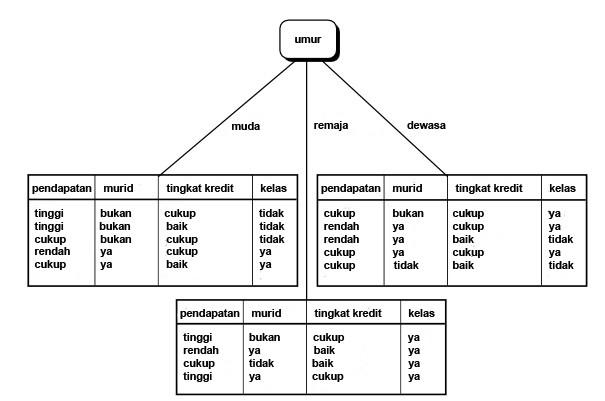
\includegraphics[scale=1]{Gambar/hasilcabangid3.jpg}
\caption[Hasil pohon faktor pada atribut \textsl{age} dari table 2.1]{Hasil cabang dari atribut \textsl{age}, Diterjemahkan dari \cite{DM}} 
\label{fig:hasilCabang}
\end{figure}

Untuk atribut yang merupakan nilai \textsl{continuous}, harus dicari nilai \textsl{split point} untuk A. Nilai-nilai dari dua angka yang bersebelahan dapat diambil nilai tengahnya untuk dijadikan \textsl{split-point}. Jika terdapat v nilai yang berbeda dari A, maka akan terdapat v-1 kemungkinan \textsl{split point}. Kemudian nilai \textsl{split point} akan dijadikan sebagai nilai pembagi, sebagai contoh: A <= \textsl{split-point} merupakan cabang pertama, dan A > \textsl{split-point} merupakan cabang kedua.

\subsubsection{C4.5}

\textsl{Information gain} akan memiliki nilai yang baik jika suatu atribut memiliki banyak nilai yang berbeda, namun hal itu tidak selalu bagus. Sebagai contoh kasus, jika nilai id suatu table yang memiliki nilai unik, maka akan terdapat banyak sekali cabang. Namun setiap cabang hanya akan berisi satu tuple dan bersifat \textsl{pure}, maka nilai \textsl{entropy} yang dihasilkan adalah 0. Oleh karena itu, informasi yang diperoleh pada atribut ini akan bernilai maksimum namun tidak akan berguna untuk \textsl{classification} \cite{DM}. Selain itu, ID3 dapat menghasil \textsl{decision tree} yang memprediksi secara berlebihan (\textsl{overestimated}) atau disebut juga \textsl{overfitting}. Hal ini dikarenakan pohon yang dihasilkan terlalu detail sehingga data input memiliki hasil prediksi yang pasti. 

C4.5 merupakan teknik lanjutan dari ID3, yang menggunakan \textsl{gain ratio} sebagai \textsl{attribute selection measure} untuk memilih atribut. Kemudian, C4.5 melakukan \textsl{tree pruning} untuk menghindari \textsl{overfitting}.

%\textsl{Information gain} akan memiliki nilai yang baik jika suatu atribut memiliki banyak nilai yang berbeda, namun hal itu tidak selalu bagus. Sebagai contoh kasus, jika nilai id suatu table yang memiliki nilai unik, maka akan terdapat banyak sekali cabang. Namun setiap cabang hanya akan berisi satu tuple dan bersifat \textsl{pure}, maka nilai \textsl{entropy} yang dihasilkan adalah 0. Oleh karena itu, informasi yang diperoleh pada atribut ini akan bernilai maksimum namun tidak akan berguna untuk \textsl{classification} \cite{DM}.

C4.5, menggunakan nilai tambahan dari \textsl{information gain} yaitu \textsl{gain ratio}, yang dapat mengatasi permasalahan \textsl{information gain} tentang nilai yang banyak. C4.5 melakukan teknik normalisasi terhadap \textsl{gain information} dengan menggunakan \textsl{split information} yang memiliki rumus sebagai berikut:

\begin{displaymath}
	SplitInfo_A(D) = - \sum_{j=1}^v \frac{|D_j|}{|D|} \times \log_2 (\frac{|D_j|}{|D|})
\end{displaymath}

Dimana |D| merupakan banyak data dan $|D_{j}|$ merupakan banyak data suatu nilai pada atribut.
Setelah mendapatkan nilai \textsl{split info} dari suatu atribut, dapat diperoleh nilai \textsl{gain ratio} dengan rumus sebagai berikut:

\begin{displaymath}
	GainRatio(A) = \frac{Gain(A)}{SplitInfo(A)}
\end{displaymath}

Nilai dari \textsl{gain ratio} terbesar yang akan dipilih. Perlu diketahui \cite{DM} jika nilai hasil mendekati 0, maka ratio menjadi tidak stabil, oleh karena itu, \textsl{gain information} yang dipilih harus besar, minimal sama besarnya dengan nilai rata-rata dari semua test yang diperiksa.

Contoh studi kasus, akan dilakukan perhitungan \textsl{gain ratio} dengan menggunakan training set pada table \ref{table:contohTrainingSet}. Dapat dilihat pada atribut pendapatan memiliki tiga partisi yaitu rendah, sedang, dan tinggi. Terdapat empat tuple dengan nilai rendah, enam tuple dengan nilai sedang, dan empat tuple dengan nilai tinggi. Untuk menghitung \textsl{gain ratio}, perlu dihitung nilai \textsl{split information} terlebih dahulu dengan cara:

\begin{displaymath}
	SplitInfo_A(D) = - \frac{4}{14} \times \log_2 (\frac{4}{14}) - \frac{6}{14} \times \log_2 (\frac{6}{14}) - \frac{4}{14} \times \log_2 (\frac{4}{14})
\end{displaymath} 
\begin{displaymath}
	SplitInfo_A(pendapatan) = 0.926 bits
\end{displaymath} 

Jika nilai \textsl{gain information} dari \textsl{income} adalah 0.029, maka, dapat diperoleh \textsl{gain ratio} dari pendapatan adalah

\begin{displaymath}
	GainRatio(pendapatan) = \frac{0.029}{0.926} = 0.031 bits
\end{displaymath}

Maka nilai \textsl{gain ratio} dari atribut pendapatan adalah 0.031 bits. Perhitungan tersebut dilakukan pada semua atribut, dan atribut yang memiliki nilai \textsl{gain ratio} yang terbesar adalah atribut yang dipilih.
\paragraph{Tree Pruning}
	
\textsl{Tree pruning} merupakan proses pemotongan \textsl{decision tree} agar lebih efisien dan tidak terlalu mempengaruhi nilai keputusan yang dihasilkan. \textsl{decision tree} yang sudah dipotong akan lebih kecil ukuran pohonnya, tidak serumit dengan pohon yang asli, namun lebih mudah untuk diproses. \textsl{Decision tree} yang sudah dipotong memiliki kecepatan serta ketepatan mengklasifikasikan yang lebih baik \cite{DM}. Perbedaan \textsl{decision tree} yang sudah dipotong dan belum dapat dilihat pada gambar \ref{fig:treePruning}.

\begin{figure}
\centering
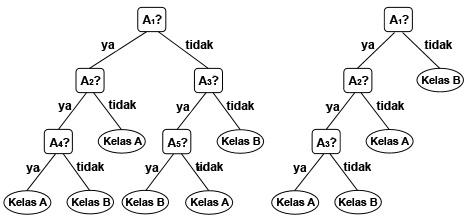
\includegraphics[scale=1]{Gambar/treepruning.jpg}
\caption[\textsl{Decision Tree Pruned}]{\textsl{Decision tree} yang belum dipotong dan yang sudah dipotong, Diterjemahkan dari \cite{DM}} 
\label{fig:treePruning}
\end{figure}

Terdapat dua pendekatan dalam melakukan \textsl{pruning}, yaitu \textsl{prepruning} dan \textsl{postpruning}.

Pada \textsl{prepruning}, pemotongan pohon dilakukan dengan cara menahan dan tidak melanjutkan pembuatan cabang atau partisi dari sebuah node, dan membuat node tersebut menjadi \textsl{leaf}. 

Pada \textsl{postpruning}, pemotongan pohon dilakukan ketika \textsl{decision tree} sudah selesai dibangun dengan cara menggubah cabang pohon menjadi \textsl{leaf}.

\subsection{\textsl{Pattern Evaluation}}
\textsl{Pattern evaluation} merupakan tahap mengidentifikasi apakah \textsl{pattern} atau pola tersebut menarik dan merepresentasikan \textsl{knowledge} berdasarkan beberapa \textsl{interestingness measures}.
Suatu \textsl{pattern} atau pola dapat dinyatakan menarik apabila
\begin{itemize}
	\item mudah dimengerti oleh manusia
	\item valid untuk data percobaan maupun data yang baru
	\item memiliki potensi atau berguna
	\item merepresentasikan \textsl{knowledge}
\end{itemize}

\subsection{\textsl{Knowledge Presentation}}
\textsl{Knowledge presentation} merupakan tahap representasi dan visualisasi terhadap \textsl{knowledge} yang merupakan hasil dari \textsl{knowledge discovery}.	
%\section{\textsl{Spatial and Spatiotemporal}}

\section{Log Histori KIRI}

KIRI memiliki log histori yang melakukan pencatatan untuk setiap user ketika menggunakan KIRI. Data log tersebut diperoleh dengan cara melakukan wawancara dengan developer KIRI, yaitu Pascal Alfadian. Data log yang diberikan sudah dalam format excel.

\textsl{Log} tersebut memiliki 5 \textsl{field} untuk setiap tuple sebagai berikut:
\begin{itemize}
	\item logId, primary key dari tuple
	\item APIKey, mengidentifikasikan sumber dari pencarian ini
	\item \textsl{Timestamp} (UTC), waktu ketika pengguna KIRI mencari rute angkot menggunakan waktu UTC / GMT
	\item \textsl{Action}, tipe dari log yang dibuat.
	\item AdditionalData, mencatat data-data yang berhubungan sesuai dengan nilai atribut\textsl{action}
\end{itemize}

LogId merupakan \textsl{field} dengan tipe data int dengan batas 6 karakter yang digunakan sebagai \textsl{primary key} dari table tersebut. LogId diisi dengan menggunakan fungsi \textsl{increment integer}. \textsl{Increment integer} merupakan fungsi untuk pengisian data pada database dengan menambahkan nilai 1 dari nilai yang terakhir kali diisi.
APIKey merupakan \textsl{field} dengan tipe data varchar yang digunakan untuk mengindentifikasi pengguna KIRI ketika menggunakan KIRI.
\textsl{Timestamp} (UTC) merupakan \textsl{field} dengan tipe data \textsl{timestamp} yang digunakan untuk mencatat waktu penggunaan KIRI oleh user, diisi dengan menggunakan fungsi \textsl{current time}. \textsl{Current time} merupakan fungsi untuk pengisian data pada database dengan mengambil waktu pada komputer ketika \textsl{record} dibuat.
\textsl{Action} merupakan \textsl{field} dengan tipe data varchar yang digunakan untuk memeriksa fungsi apa yang dipanggil dari API KIRI. Terdapat beberapa tipe pada \textsl{field action}, yaitu
\begin{itemize}
	\item \textsl{ADDAPIKEY}, \textsl{action} yang dicatat ke dalam log ketika fungsi pembuatan \textsl{API key} yang baru dipanggil.
	\item \textsl{FINDROUTE}, \textsl{action} yang dicatat ketika user melakukan pencarian rute
	\item \textsl{LOGIN}, \textsl{action} yang dicatat ketika developers melakukan login dengan menggunakan \textsl{API key}
	\item \textsl{NEARBYTRANSPORT}, \textsl{action} yang dicatat ketika user mencari transportasi di daerah rute sedang dicari
	\item \textsl{PAGELOAD}, \textsl{action} yang dicatat ketika user memasuki halaman KIRI
 	\item \textsl{REGISTER},\textsl{action} yang dicatat ketika developers melakukan pendaftaran pada KIRI \textsl{API key}
	\item \textsl{SEARCHPLACE}, \textsl{action} yang dicatat ketika user memanggil fungsi pencarian lokasi dengan menggunakan nama tempat
	\item \textsl{WIDGETERROR}, mencatat log tersebut ketika user menerima error dari \textit{widget}
	\item \textsl{WIDGETLOAD}, mencatat log tersebut ketika user melakukan download widget
\end{itemize}
AdditionalData, merupakan \textsl{field} dengan tipe data varchar yang digunakan untuk mencatat informasi yang dibutuhkan sesuai dengan \textsl{field action}. Isi dari additionalData tersebut untuk setiap \textsl{action} adalah
\begin{itemize}
	\item Jika nilai atribut \textsl{action} adalah \textsl{ADDAPIKEY}, maka isi nilai dari additionalData adalah nilai \textsl{API key} yang dihasilkan
	\item Jika nilai atribut \textsl{action} adalah \textsl{FINDROUTE}, maka isi nilai dari additionalData adalah \textsl{latitude} dan \textsl{longitude} lokasi awal dan tujuan serta banyak jalur yang dihasilkan dari aplikasi KIRI
	\item Jika nilai atribut \textsl{action} adalah \textsl{LOGIN}, maka isi nilai dari additionalData adalah id dari user yang melakukan login serta status apakah user berhasil login atau tidak
	\item Jika nilai atribut \textsl{action} adalah \textsl{NEARBYTRANSPORT}, maka isi dari additionalData adalah \textsl{latitude} dan \textsl{longitude} dari transportasi tersebut
	\item Jika nilai atribut \textsl{action} adalah \textsl{PAGELOAD}, maka isi nilai dari additionalData adalah ip dari user
	\item Jika nilai atribut \textsl{action} adalah \textsl{REGISTER}, maka isi nilai dari additionalData adalah alamat email yang digunakan untuk meregister dan nama user
	\item Jika nilai atribut \textsl{action} adalah \textsl{SEARCHPLACE}, maka isi nilai dari additionalData adalah nama tempat yang dicari
	\item Jika nilai atribut \textsl{action} adalah \textsl{WIDGETERROR}, maka isi nilai dari additionalData adalah isi pesan dari error yang terjadi
	\item Jika nilai atribut \textsl{action} adalah \textsl{WIDGETLOAD}, maka isi nilai dari additionalData adalah ip dari user yang melakukan download widget
\end{itemize}

\section{\textsl{Haversine Formula}}\cite{Haversine}
\textsl{Haversine Formula} dapat menghasilkan nilai jarak antar dua titik pada bola dari garis bujur dan garis lintang titik tersebut. Berikut rumus Haversine:

\begin{displaymath}
	a = \sin^{2}((|\varphi_{1}-\varphi_{2}|)/2) + \cos\varphi_{1} . \cos\varphi_{2} . \sin^{2}((|\lambda_{1}-\lambda_{2}|)/2)
\end{displaymath}
\begin{displaymath}
	c = 2 . a\tan^{2}(\sqrt{a}, \sqrt{1-a})
\end{displaymath}
\begin{displaymath}
	d = R . c
\end{displaymath}

Dimana 
\begin{itemize}
	\item $\varphi$ adalah latitude dalam radian
	\item $\lambda$ adalah longitude dalam radian
	\item R adalah radius bumi (radius = 6,371km)
\end{itemize}

Contoh untuk perhitungan Haversine sebagai berikut:
Jika kita ingin menghitung jarak dua titik dari daerah Jakarta ke Surabaya, dengan titik pada Jakarta adalah -6.211544, 106.845172 dan titik pada Surabaya adalah -7.289166, 112.734398, maka perhitungan rumusnya akan menjadi

\begin{displaymath}
	a = \sin^{2}((|-6.211544-(-7.289166)|)/2) + \cos-6.211544 . \cos-7.289166 . \sin^{2}((|106.845172-112.734398|)/2)
\end{displaymath}
\begin{displaymath}
	a = 0.0026906745
\end{displaymath}

\begin{displaymath}
	c = 2 . 0.0026906745\tan^{2}(\sqrt{0.0026906745}, \sqrt{1-0.0026906745})
\end{displaymath}
\begin{displaymath}
	c =  0.1037900036
\end{displaymath}

\begin{displaymath}
	d = 6.371 X 0.1037900036
\end{displaymath}
\begin{displaymath}
	d = 0.6612461130 * 1000 km
\end{displaymath}
\begin{displaymath}
	d = 661.2461130 km
\end{displaymath}

Dengan menggunakan rumus Haversine, maka jarak antar kedua titik tersebut adalah 661.246 km

\section{Weka}\cite{Weka}
Weka merupakan aplikasi berbasis java yang berisi alat-alat untuk melakukan visualisasi dan algoritma untuk data analisis serta pemodelan prediksi. Weka juga menyediakan file weka-src.jar yang berisi kelas-kelas yang dipakai oleh aplikasi weka sehingga user dapat menggunakannya untuk membuat program java yang berfungsi untuk \textsl{data mining}. Berikut beberapa kelas yang dimiliki oleh Weka:

\paragraph{\textsl{Classifier}} adalah sebuah \textsl{interface} yang digunakan sebagai skema untuk prediksi numerik ataupun nominal pada weka. Kelas tersebut memiliki \textsl{method} sebagai berikut:
\begin{itemize}
	
	\item void buildClassifier(Instances data)
	
	untuk melakukan menghasilkan klasifikasi dengan parameter set data pelatihan.
	
	\item double classfyInstance(Instances instance)
	
	untuk melakukan klasifikasi dari data dengan parameter contoh data yang akan dilakukan klasifikasi. Method tersebut akan mengebalikan nilai kelas yang sesuai dengan data tersebut.
	
	\item double[] distributionForInstance(Instance instance)
	
	untuk memprediksi keanggotaan kelas untuk contoh yang diberikan dengan parameter contoh data yang akan dilakukan klasifikasi dan mengembalikan array yang berisi nilai keanggotaan dari contoh data.
	
	\item Capabilities getCapabilities()
	
	mengembalikan capabilities dari kelas tersebut.
\end{itemize}

\paragraph{Instance} adalah interface yang mewakili set data.


Method:
\begin{itemize}
	\item Attribute attribute(int index)
	
	Mengembalikan atribut dari indeks yang diberikan.
	
	\item Attribute classAttribute()
	
	Mengembalikan atribut kelas.
	
	\item int classIndex()
	
	Mengembalikan indeks atribut kelas itu.
	
	\item boolean classIsMissing()
	
	Mengecek apakah kelas turunan hilang.
	
	\item double classValue()
	
	Mengembalikan nilai kelas contoh sebagai angka floating-point.
	
	\item Instances dataset()
	
	Mengembalikan dataset.
	
	\item void deleteAttributeAt(int position)
	
	Menghapus atribut pada posisi tertentu.
	
	\item java.util.Enumeration<Attribute> enumerateAttributes()
	
	Mengembalikan penghitungan semua atribut.
	
	\item boolean equalHeaders(Instance inst)
	
	Pengujian jika header dari dua contoh yang setara.
	
	\item java.lang.String equalHeadersMsg(Instance inst)
	
	Memeriksa apakah header dari dua contoh yang setara.
	
	\item boolean hasMissingValue()
	
	Tes apakah sebuah contoh memiliki nilai yang hilang.
	
	\item index(int position)
	
	Mengembalikan index dari atribut yang tersimpan di posisi tertentu.
	
	\item void insertAttributeAt(int position)
	
	Menyisipkan atribut pada posisi tertentu.
	
	\item boolean isMissing(Attribute att)
	
	Pengujian jika nilai tertentu yang hilang.
	
	\item boolean isMissing(int attIndex)
	
	Pengujian jika nilai tertentu yang hilang.
	
	\item boolean isMissingSparse(int indexOfIndex)
	
	Pengujian jika nilai tertentu yang hilang.
	
	\item Instance mergeInstance(Instance inst)
	
	Menggabungkan contoh yang diberikan dan mengembalikan hasilnya.
	
	\item int numAttributes()
	
	Mengembalikan jumlah atribut.
	
	\item int numClasses()
	
	Mengembalikan jumlah label kelas.
	
	\item int numValues()
	
	Mengembalikan jumlah nilai.
	
	\item Instances relationalValue(Attribute att)
	
	Mengembalikan nilai relasional atribut relasional.
	
	\item Instances relationalValue(int attIndex)
	
	Mengembalikan nilai relasional atribut relasional.
	
	\item void replaceMissingValues(double[] array)
	
	Menggantikan semua nilai yang hilang dalam contoh dengan nilai-nilai yang terkandung dalam array yang diberikan.
	
	\item void setClassMissing()
	
	Menetapkan nilai kelas contoh untuk hilang.
	
	\item void setClassValue(double value)
	
	Menetapkan nilai kelas turunan dengan nilai yang diberikan (format floating-point).
	
	\item void setClassValue(java.lang.String value)
	
	Menetapkan nilai kelas turunan dengan nilai yang diberikan.
	
	\item void setDataset(Instances instances)
	
	Mengatur referensi dataset.
	
	\item void setMissing(Attribute att)
	
	Menetapkan nilai tertentu dijadikan hilang.
	
	\item void setMissing(int attIndex)
	
	Menetapkan nilai tertentu dijadikan hilang.
	
	\item void setValue(Attribute att, double value)
	
	Menetapkan nilai tertentu dalam hal untuk nilai yang diberikan (format floating-point).
	
	\item void setValue(Attribute att, java.lang.String value)
	
	Menetapkan nilai atribut nominal atau string ke nilai yang diberikan.
	
	\item void setValue(int attIndex, double value)
	
	Menetapkan nilai tertentu untuk nilai yang diberikan (format floating-point).
	
	\item void setValue(int attIndex, java.lang.String value)
	
	Menetapkan nilai atribut nominal atau string ke nilai yang diberikan.
	
	\item void setValueSparse(int indexOfIndex, double value)
	
	Menetapkan nilai tertentu dalam contoh dengan nilai yang diberikan (format floating-point).
	
	\item void setWeight(double weight)
	
	Mengatur berat contoh.
	
	\item java.lang.String stringValue(Attribute att)
	
	Mengembalikan nilai nominal, string, tanggal, atau atribut relasional untuk contoh sebagai string.
	
	\item java.lang.String stringValue(int attIndex)
	
	Mengembalikan nilai nominal, string, tanggal, atau atribut relasional untuk contoh sebagai string.
	
	\item double[] toDoubleArray()
	
	Mengembalikan nilai-nilai masing-masing atribut sebagai array ganda.
	
	\item java.lang.String toString(Attribute att)
	
	Mengembalikan deskripsi satu nilai dari contoh sebagai string.
	
	\item java.lang.String toString(Attribute att, int afterDecimalPoint)
	
	Mengembalikan deskripsi satu nilai dari contoh sebagai string.
	
	\item java.lang.String toString(int attIndex)
	
	Mengembalikan deskripsi satu nilai dari contoh sebagai string.
	
	\item java.lang.String toString(int attIndex, int afterDecimalPoint)
	
	Mengembalikan deskripsi satu nilai dari contoh sebagai string.
	
	\item java.lang.String toStringNoWeight()
	
	Mengembalikan deskripsi satu contoh (tanpa berat ditambahkan).
	
	\item double value(Attribute att)
	
	Mengembalikan nilai atribut contoh dalam format internal.
	
	\item double value(int attIndex)
	
	Mengembalikan nilai atribut contoh dalam format internal.
	
	\item double valueSparse(int indexOfIndex)
	
	Mengembalikan nilai atribut contoh dalam format internal.
	
	\item double weight()
	
	Mengembalikan berat contoh itu.
\end{itemize}

\paragraph{Instances} adalah kelas untuk menangani set data.

Atribut:
\begin{itemize}
	
	\item String ARFF\_DATA
	
	digunakan untuk menunjukkan section arff data.
	
	\item String ARFF\_RELATION
	
	digunakan untuk menunjukkan header arff data.
	
	\item String FILE\_EXTENSION
	
	extension dari nama file yang digunakan untuk file arff.
	
	\item String SERIALIZED\_OBJ\_FILE\_EXTENSION
	
	ektension dari nama file yang digunakan untuk \textsl{bin}.
\end{itemize}

\textsl{Constructor}:
\begin{itemize}
	\item Instances(Instances dataset)
	
	Konstruktor menyalin semua contoh dan referensi untuk informasi header dari himpunan contoh.
	
	\item Instances(Instances dataset, int capacity)
	
	
	Konstruktor menciptakan himpunan kosong contoh.
	
	\item Instances(Instances source, int first, int toCopy)
	
	Menciptakan satu set baru kasus dengan menyalin bagian dari satu set.
	
	\item Instances(java.io.Reader reader)
	
	Membaca file ARFF, dan memberikan bobot satu untuk setiap contoh.
	
	\item Instances(java.lang.String name, java.util.ArrayList<Attribute> attInfo, int capacity)
	
	Menciptakan himpunan kosong contoh.
\end{itemize}

\textsl{Method}:
\begin{itemize}
	\item boolean add(Instance instance)
	
	Menambahkan set data.
	
	\item void add(int index, Instance instance)
	
	Menambahkan satu contoh di posisi tertentu dalam daftar.
	
	\item Attribute attribute(int index)
	
	Mengembalikan atribut.
	
	\item Attribute attribute(java.lang.String name)
	
	Mengembalikan atribut yang sesuai dengan nama yang diberikan.
	
	\item AttributeStats attributeStats(int index)
	
	Menghitung ringkasan statistik pada nilai-nilai yang muncul dalam rangkaian kasus untuk atribut tertentu.
	
	\item double[] attributeToDoubleArray(int index)
	
	Mendapat nilai semua contoh dalam dataset ini untuk atribut tertentu.
	
	\item boolean checkForAttributeType(int attType)
	
	Cek untuk atribut dari tipe yang diberikan dalam dataset.
	
	\item boolean checkForStringAttributes()
	
	Cek string atribut dalam dataset.
	
	\item boolean checkInstance(Instance instance)
	
	Memeriksa apakah contoh yang diberikan kompatibel dengan dataset ini.
	
	\item Attribute classAttribute()
	
	Mengembalikan atribut class.
	
	\item int classIndex()
	
	Mengembalikan indeks atribut kelas itu.
	
	\item void delete()
	
	Menghapus semua contoh dari set.
	
	\item void delete(int index)
	
	Menghapus sebuah contoh di posisi tertentu dari set.
	
	\item void deleteAttributeAt (int position)
	
	Menghapus atribut pada posisi tertentu. %(position sampai numAttributes () - 1).
	
	\item void deleteAttributeType(int attType)
	
	Menghapus semua atribut dari tipe yang diberikan dalam dataset.
	
	\item void deleteStringAttributes()
	
	Menghapus semua atribut string dalam dataset.
	
	\item void deleteWithMissing(Attribute att)
	
	Menghapus semua contoh dengan nilai-nilai yang hilang untuk atribut tertentu dari dataset.
	
	\item void deleteWithMissing(int attIndex)
	
	Menghapus semua contoh dengan nilai-nilai yang hilang untuk atribut tertentu dari dataset.
	
	\item void deleteWithMissingClass()
	
	Menghapus semua contoh dengan nilai kelas hilang dari dataset.
	
	\item java.util.Enumeration<Attribute> enumerateAttributes()
	
	Pengembalian penghitungan semua atribut.
	
	\item java.util.Enumeration<Instance> enumerateInstances()
	
	Pengembalian penghitungan semua contoh dalam dataset.
	
	\item boolean equalHeaders(Instances dataset)
	
	Cek jika dua header yang setara.
	
	\item java.lang.String equalHeadersMsg(Instances dataset)
	
	Cek jika dua header yang setara.
	
	\item Instance firstInstance()
	
	Mengembalikan contoh pertama di set.
	
	\item Instance get(int index)
	
	Mengembalikan contoh pada posisi tertentu.
	
	\item java.util.Random getRandomNumberGenerator(long seed)
	
	Mengembalikan nomor acak.
	
	\item java.lang.String getRevision()
	
	Mengembalikan string revisi.
	
	\item void insertAttributeAt(Attribute att, int position)
	
	Menyisipkan atribut pada posisi tertentu (0 numAttributes ()) dan menetapkan semua nilai hilang.
	
	\item Instance instance(int index)
	
	Mengembalikan contoh pada posisi tertentu.
	
	\item double kthSmallestValue(Attribute att, int k)
	
	Mengembalikan nilai atribut k-terkecil dari atribut numerik.
	
	\item double kthSmallestValue(int attIndex, int k)
	
	Mengembalikan nilai atribut k-terkecil dari atribut numerik.
	
	\item Instance lastInstance()
	
	Mengembalikan contoh terakhir di set.
	
	\item static void main(java.lang.String[] args)
	
	Metode utama untuk kelas ini.
	
	\item double meanOrMode(Attribute att)
	
	Mengembalikan rata (mode) untuk angka (nominal) atribut sebagai nilai floating-point.
	
	\item double meanOrMode(int attIndex)
	
	Mengembalikan rata (mode) untuk angka (nominal) atribut sebagai nilai floating-point.
	
	\item static Instances mergeInstances(Instances first, Instances second)
	
	Menggabungkan dua set Contoh bersama-sama
	
	\item int numAttributes()
	
	Mengembalikan jumlah atribut.
	
	\item int numClasses()
	
	Mengembalikan jumlah label kelas.
	
	\item int numDistinctValues(Attribute att)
	
	Mengembalikan jumlah nilai yang berbeda dari atribut yang diberikan.
	
	\item int numDistinctValues(int attIndex)
	
	Mengembalikan jumlah nilai yang berbeda dari atribut yang diberikan.
	
	\item int numInstances()
	
	Mengembalikan jumlah kasus dalam dataset.
	
	\item void randomize(java.util.Random random)
	
	Mengocok contoh di set sehingga mereka memerintahkan secara acak.
	
	\item java.lang.String relationName()
	
	Mengembalikan nama hubungan itu.
	
	\item Instance remove(int index)
	
	Menghapus contoh pada posisi tertentu.
	
	\item void renameAttribute(Attribute att, java.lang.String name)
	
	Mengganti nama atribut.
	
	\item void renameAttribute(int att, java.lang.String name)
	
	Mengganti nama atribut.
	
	\item void renameAttributeValue(Attribute att, java.lang.String val, java.lang.String name)
	
	Mengganti nama nilai nominal (atau string) nilai atribut
	
	\item void renameAttributeValue(int att, int val, java.lang.String name)
	
	Mengganti nama nilai nominal (atau string) nilai atribut.
	
	\item void replaceAttributeAt(Attribute att, int position)
	
	Menggantikan atribut pada posisi tertentu (0 numAttributes ()) dengan atribut yang diberikan dan menetapkan semua nilai yang hilang.
	
	\item Instances resample(java.util.Random random)
	
	Membuat dataset baru dengan ukuran yang sama dengan menggunakan random sampling dengan penggantian.
	
	\item Instances resampleWithWeights(java.util.Random random)
	
	Membuat dataset baru dengan ukuran yang sama dengan menggunakan random sampling dengan penggantian sesuai dengan contoh berat saat ini.
	
	\item Instances resampleWithWeights(java.util.Random random, boolean representUsingWeights)
	
	Membuat dataset baru dengan ukuran yang sama dengan menggunakan random sampling dengan penggantian sesuai dengan contoh berat saat ini.
	
	\item Instances resampleWithWeights(java.util.Random random, boolean[] sampled)
	
	Membuat dataset baru dengan ukuran yang sama dengan menggunakan random sampling dengan penggantian sesuai dengan contoh berat saat ini.
	
	\item Instances resampleWithWeights(java.util.Random random, boolean[] sampled, boolean representUsingWeights)
	
	Membuat dataset baru dengan ukuran yang sama dengan menggunakan random sampling dengan penggantian sesuai dengan contoh berat saat ini.
	
	\item Instances resampleWithWeights(java.util.Random random, double[] weights)
	
	Membuat dataset baru dengan ukuran yang sama dengan menggunakan random sampling dengan penggantian sesuai dengan vektor bobot yang diberikan.
	
	\item Instances resampleWithWeights(java.util.Random random, double[] weights, boolean[] sampled)
	
	Membuat dataset baru dengan ukuran yang sama dengan menggunakan random sampling dengan penggantian sesuai dengan vektor bobot yang diberikan.
	
	\item Instances resampleWithWeights(java.util.Random random, double[] weights, boolean[] sampled, boolean representUsingWeights)
	
	Membuat dataset baru dengan ukuran yang sama dengan menggunakan random sampling dengan penggantian sesuai dengan vektor bobot yang diberikan.

	\item Instance set(int index, Instance instance)

	Menggantikan contoh pada posisi tertentu.
	
	\item void setClass(Attribute att)
	
	Mengatur atribut class.
	
	\item void setClassIndex(int classIndex)
	
	Mengatur indeks kelas set.
	
	\item void setRelationName(java.lang.String newName)
	
	Mengatur nama hubungan itu.
	
	\item int size()
	
	Mengembalikan banyak data dalam dataset.
	
	\item void sort(Attribute att)
	
	Urutkan contoh berdasarkan atribut.
	
	\item void sort(int attIndex)
	
	Urutkan contoh berdasarkan atribut.
	
	\item void stableSort(Attribute att)
	
	Urutkan contoh berdasarkan atribut, menggunakan semacam stabil.
	
	\item void stableSort(int attIndex)
	
	Urutkan contoh berdasarkan atribut, menggunakan semacam stabil
	
	\item void stratify(int numFolds)
	
	Mengelompokkan satu set contoh sesuai dengan nilai-nilai kelasnya jika atribut kelas nominal (sehingga setelah cross-validasi berlapis dapat dilakukan).
	
	\item Instances stringFreeStructure()
	
	Buat salinan struktur. 
	
	\item double sumOfWeights()
	
	Menghitung jumlah semua bobot contoh.
	
	\item void swap(int i, int j)
	
	menukar posisi dua contoh di set.
	
	\item static void test(java.lang.String[] argv)
	
	Metode pengujian kelas ini.
	
	\item Instances testCV(int numFolds, int numFold)
	
	Menciptakan set tes untuk satu kali lipat dari cross-validasi pada dataset.
	
	\item java.lang.String toString()
	
	Mengembalikan dataset sebagai string dalam format ARFF.
	
	\item java.lang.String toSummaryString()
	
	Menghasilkan string meringkas set contoh
	
	\item Instances trainCV(int numFolds, int numFold)
	
	Menciptakan pelatihan ditetapkan untuk satu kali lipat dari cross-validasi pada dataset.
	
	\item Instances trainCV(int numFolds, int numFold, java.util.Random random)
	
	Menciptakan pelatihan ditetapkan untuk satu kali lipat dari cross-validasi pada dataset.
	
	\item double variance(Attribute att)
	
	Menghitung varians untuk atribut numerik.
	
	\item double variance(int attIndex)
	
	Menghitung varians untuk atribut numerik.
	
	\item double[] variances()
	
	Menghitung varians untuk semua atribut numerik secara bersamaan.
\end{itemize}

\paragraph{Attribute} adalah kelas yang digunakan untuk menangani atribut.

\textsl{Atribut}:
\begin{itemize}
	\item static java.lang.String ARFF\_ATTRIBUTE
	
	Kata kunci yang digunakan untuk menunjukkan awal atribut deklarasi ARFF.
	
	\item static java.lang.String ARFF\_ATTRIBUTE\_DATE
	
	Kata kunci yang digunakan untuk menunjukkan tanggal atribut.
	
	\item static java.lang.String ARFF\_ATTRIBUTE\_INTEGER
	
	Kata kunci yang digunakan untuk menunjukkan atribut numerik.
	
	\item static java.lang.String ARFF\_ATTRIBUTE\_NUMERIC
	
	Kata kunci yang digunakan untuk menunjukkan atribut numerik.
	
	\item static java.lang.String ARFF\_ATTRIBUTE\_REAL
	
	Kata kunci yang digunakan untuk menunjukkan atribut numerik.
	
	\item static java.lang.String ARFF\_ATTRIBUTE\_RELATIONAL
	
	Kata kunci yang digunakan untuk menunjukkan atribut relasi bernilai.
	
	\item static java.lang.String ARFF\_ATTRIBUTE\_STRING
	
	Kata kunci yang digunakan untuk menunjukkan atribut String.
	
	\item static java.lang.String ARFF\_END\_SUBRELATION
	
	Kata kunci yang digunakan untuk menunjukkan akhir dari deklarasi subrelation.
	
	\item static int DATE
	
	Set konstan untuk atribut dengan nilai tanggal.
	
	\item static java.lang.String DUMMY\_STRING\_VAL
	
	Dummy pertama nilai String atribut.
	
	\item static int NOMINAL
	
	Set konstan untuk atribut nominal.
	
	\item static int NUMERIC
	
	Set konstan untuk atribut numerik.
	
	\item static int ORDERING\_MODULO
	
	Set konstan untuk atribut ordering modulo.
	
	\item static int ORDERING\_ORDERED
	
	Set konstan untuk atribut memerintahkan.
	
	\item static int ORDERING\_SYMBOLIC
	
	Set konstan untuk atribut simbolik.
	
	\item static int RELATIONAL
	
	Set konstan untuk atribut nilai relasi.
	
	\item static int STRING
	
	Set konstan untuk atribut dengan nilai-nilai string.
\end{itemize}
\textsl{Constructor}:
\begin{itemize}
	\item Attribute(java.lang.String attributeName)
	
	Konstruktor untuk atribut numerik.
	
	\item Attribute(java.lang.String attributeName, Instances header)
	
	Konstruktor untuk atribut nilai relasi.
	
	\item Attribute(java.lang.String attributeName, Instances header, int index)
	
	Konstruktor untuk atribut nilai relasi dengan indeks tertentu.
	
	\item Attribute(java.lang.String attributeName, Instances header, ProtectedProperties metadata)
	
	Konstruktor untuk atribut nilai relasi.
	
	\item Attribute(java.lang.String attributeName, int index)
	
	Konstruktor untuk atribut numerik dengan indeks tertentu.
	
	\item Attribute(java.lang.String attributeName, java.util.List<java.lang.String> attributeValues)
	
	Konstruktor untuk atribut nominal dan atribut string.
	
	\item Attribute(java.lang.String attributeName, java.util.List<java.lang.String> attributeValues, int index)
	
	Konstruktor untuk atribut nominal dan atribut string dengan indeks tertentu.
	
	\item Attribute(java.lang.String attributeName, java.util.List<java.lang.String> attributeValues, ProtectedProperties metadata)
	
	Konstruktor untuk atribut nominal dan atribut string, di mana metadata diberikan.
	
	\item Attribute(java.lang.String attributeName, ProtectedProperties metadata)
	
	Konstruktor untuk atribut numerik, di mana metadata diberikan.
	
	\item Attribute(java.lang.String attributeName, java.lang.String dateFormat)
	
	Konstruktor untuk tanggal atribut.
	
	\item Attribute(java.lang.String attributeName, java.lang.String dateFormat, int index)
	
	Konstruktor untuk tanggal atribut dengan indeks tertentu.
	
	\item Attribute(java.lang.String attributeName, java.lang.String dateFormat, ProtectedProperties metadata)
	
	Konstruktor untuk atribut tanggal, di mana metadata diberikan.
\end{itemize}
\textsl{Method}:
\begin{itemize}
	\item int addRelation(Instances value)
	
	Menambahkan relasi pada atribut nilai relasi.
	
	\item int addStringValue(Attribute src, int index)
	
	Menambahkan nilai string ke daftar string yang valid untuk atribut jenis string dan mengembalikan indeks string.
	
	\item int addStringValue(java.lang.String value)
	
	Menambahkan nilai string ke daftar string yang valid untuk atribut jenis string dan mengembalikan indeks string
	
	\item java.lang.Object copy()
	
	Menghasilkan salinan atribut ini.
	
	\item Attribute copy(java.lang.String newName)
	
	Menghasilkan salinan atribut ini dengan nama baru.
	
	\item java.util.Enumeration<java.lang.Object> enumerateValues()
	
	Pengembalian penghitungan semua nilai atribut jika atribut nominal, string, atau hubungan-nilai, null sebaliknya.
	
	\item boolean equals(java.lang.Object other)
	
	Pengujian jika diberikan atribut sama dengan atribut ini.
	
	\item java.util.String equalsMsg(java.lang.Object other)
	
	Pengujian jika diberikan atribut sama dengan atribut ini.
	
	\item java.util.String formatDate(double date)
	
	Mengembalikan milidetik sesuai dengan tanggal saat ini.
	
	\item java.util.String getDateFormat()
	
	Mengembalikan pola format tanggal dalam hal atribut ini adalah tipe date, selain itu, maka string akan kosong.
	
	\item double getLowerNumericBound()
	
	Pengembalian batas bawah dari atribut numerik.
	
	\item ProtectedProperties getMetadata()
	
	Mengembalikan properties disediakan untuk atribut ini.
	
	\item java.lang.String getRevision()
	
	Mengembalikan string revisi.
	
	\item double getUpperNumericBound()
	
	Mengembalikan nilai dari atribut numerik.
	
	\item int hashCode()
	
	Mengembalikan kode hash untuk atribut ini berdasarkan namanya.
	
	\item boolean hasZeropoint()
	
	Pengembalian apakah atribut memiliki zeropoint.
	
	\item int index()
	
	Mengembalikan index dari atribut ini.
	
	\item int indexOfValue(java.lang.String value)
	
	Mengembalikan index dari nilai atribut tertentu.
	
	\item boolean isAveragable()
	
	Pengembalian apakah atribut dapat dirata-ratakan bermakna.
	
	\item boolean isDate()
	
	Pengujian jika atribut adalah jenis tanggal.
	
	\item boolean isInRange(double value)
	
	Menentukan apakah suatu nilai terletak dalam batas-batas atribut.
	
	\item boolean isNominal()
	
	Menguji apakah atribut nominal.
	
	\item boolean isNumeric()
	
	Pengujian jika atribut numerik.
	
	\item boolean isRelationValued()
	
	Pengujian jika atribut hubungan dihargai.
	
	\item boolean isString()
	
	Pengujian jika atribut string.
	
	\item static void main(java.lang.String[] ops)
	
	Metode utama yang sederhana untuk menguji kelas ini.
	
	\item java.lang.String name()
	
	Mengembalikan nama atribut itu.
	
	\item int numValues()
	
	Mengembalikan jumlah nilai atribut.
	
	\item int ordering()
	
	Mengembalikan pemesanan atribut.
	
	\item int parseDate(java.lang.String string)
	
	Mengurai string yang diberikan sebagai date, sesuai format saat ini dan mengembalikan sesuai dengan jumlah milidetik.
	
	\item Instances relation()
	
	Mengembalikan informasi header untuk atribut nilai relasi, null jika atribut tidak memiliki hubungan.
	
	\item Instances relation(int valIndex)
	
	Mengembalikan nilai atribut nilai relasi.
	
	\item void setStringValue(java.lang.String value)
	
	Mengosongkan nilai dan mengatur mereka mengandung hanya nilai yang diberikan.
	
	\item void setWeight(double value)
	
	Mengatur berat atribut baru.
	
	\item java.lang.String toString()
	
	Pengembalian deskripsi atribut ini dalam format ARFF.
	
	\item int type()
	
	Mengembalikan jenis atribut sebagai integer.
	
	\item static java.lang.String typeToString(Attribute att)
	
	Mengembalikan representasi string dari jenis atribut.
	
	\item static java.lang.String typeToString(int type)
	
	Mengembalikan representasi string dari jenis atribut.
	
	\item static java.lang.String typeToStringShort(Attribute att)
	
	Mengembalikan representasi string jenis atribut.
	
	\item static java.lang.String typeToStringShort(int type)
	
	Mengembalikan representasi string jenis atribut.
	
	\item java.lang.String value(int valIndex)
	
	Mengembalikan nilai atribut nominal atau tali.
	
	\item double weight()
	
	Mengembalikan berat badan atribut itu
	
\end{itemize}
\paragraph{ID3} adalah kelas yang digunakan untuk membangun \textsl{decision tree} yang berbasis pada algoritma ID3, hanya dapat menerima input dengan atribut nominal.
\textsl{Constructor}:
\begin{itemize}
	\item ID3()
\end{itemize}
\textsl{Method}:
\begin{itemize}
	\item void buildClassifier(Instances data)
	
	Membangun ID3 pohon keputusan classifier.
	
	\item double classifyInstance(Instance instance)
	
	Mengklasifikasikan tes data yang diberikan dengan menggunakan pohon keputusan.
	
	\item double[] distributionForInstance(Instance instance)
	
	Menghitung distribusi kelas instance menggunakan pohon keputusan.
	
	\item Capabilities getCapabilities()
	
	Mengembalikan default classifier.
	
	\item java.lang.String getRevision()
	
	Mengembalikan String revisi.
	
	\item TechnicalInformation getTechnicalInformation()
	
	Mengembalikan sebuah instance dari objek TechnicalInformation, yang berisi informasi rinci tentang latar belakang teknis kelas ini.
	
	\item java.lang.String globalInfo()
	
	Mengembalikan string yang menjelaskan classifier.
	
	\item static void main(java.lang.String[] args)
	
	Metode utama untuk kelas ini.
	
	\item java.lang.String toSource(java.lang.String className)
	
	Mengembalikan string yang menggambarkan classifier.
	
	\item java.lang.String toString()
	
	Mencetak pohon keputusan menggunakan metode toString.	
\end{itemize}

\paragraph{J48} adalah kelas yang digunakan untuk membuat \textsl{decision tree} c4.5.

\textsl{Constructor}:
\begin{itemize}
	\item ID3()
\end{itemize}
\textsl{Method}:
\begin{itemize}
	\item java.lang.String binarySplitsTipText()
	
	Mengembalikan teks tip untuk properti ini.
	
	\item void buildClassifier(Instances instances)
	
	Menghasilkan classifier.
	
	\item double classifyInstance(Instance instance)
	
	Mengklasifikasikan set data.
	
	\item java.lang.String confidenceFactorTipText()
	
	Mengembalikan teks tip untuk properti ini.
	
	\item double[] distributionForInstance(Instance instance)
	
	Pengembalian probabilitas kelas untuk sebuah data.
	
	\item java.util.Enumeration enumerateMeasures()
	
	Pengembalian penghitungan ukuran.
	
	\item boolean getBinarySplits()
	
	Dapatkan nilai binarySplits.
	
	\item Capabilities getCapabilities()
	
	Mengembalikan capabilities dari kelas ini.
	
	\item float getConfidenceFactor()
	
	Mengembalikan nilai \textsl{confident}.
	
	\item double getMeasure(java.lang.String additionalMeasureName)
	
	Mengembalikan nilai bobot sesuai nama.
	
	\item int getMinNumObj()
	
	Dapatkan nilai minNumObj.
	
	\item int getNumFolds()
	
	Dapatkan nilai numFolds.
	
	\item java.lang.String getOptions()
	
	Mendapat pengaturan saat ini.
	
	\item boolean getReducedErrorPruning()
	
	Dapatkan nilai reducedErrorPruning.
	
	\item java.lang.String getRevision()
	
	Mengembalikan string revisi.
	
	\item boolean getSaveInstanceData()
	
	Periksa apakah contoh data disimpan.
	
	\item int getSeed()
	
	Dapatkan nilai seed
	
	\item boolean getSubtreeRaising()
	
	Dapatkan nilai subtreeRaising.
	
	\item TechnicalInformation getTechnicalInformation()
	
	Mengembalikan sebuah instance dari objek TechnicalInformation, yang berisi informasi rinci tentang latar belakang teknis kelas ini.

	\item boolean getUnpruned()
	
	mengecek apakah dilakukan \textsl{tree pruning}.
	
	\item boolean getUseLaplace()
	
	Dapatkan nilai useLaplace.
	
	\item java.lang.String globalInfo()
	
	Mengembalikan string yang menjelaskan classifier.
	
	\item java.lang.String graph()
	
	Pengembalian Grafik menggambarkan pohon.
	
	\item int graphType()
	
	Mengembalikan jenis grafik classifier.
	
	\item static void main(java.lang.String[] argv)
	
	Metode utama untuk menguji kelas ini.
	
	\item double measureNumLeaves()
	
	Mengembalikan jumlah daun.
	
	\item double measureNumRules()
	
	Mengembalikan sejumlah aturan.
	
	\item double measureTreeSize()
	
	Mengembalikan ukuran pohon.
	
	\item java.lang.String minNumObjTipText()
	
	Mengembalikan teks tip untuk properti ini.
	
	\item java.lang.String numFoldsTipText()
	
	Mengembalikan teks tip untuk properti ini
	
	\item java.lang.String prefix()
	
	Pengembalian pohon dalam rangka awalan.
	
	\item java.lang.String reducedErrorPruningTipText()
	
	Mengembalikan teks tip untuk properti ini
	
	\item java.lang.String saveInstanceDataTipText()
	
	Mengembalikan teks tip untuk properti ini.
	
	\item java.lang.String seedTipText()
	
	Mengembalikan teks tip untuk properti ini
	
	\item void setBinarySplits(boolean v)
	
	Mengatur nilai binarySplits.
	
	\item void setConfidenceFactor(float v)
	
	Mengatur nilai \textsl{confident}.
	
	\item void setMinNumObj(int v)
	
	Mengatur nilai minNumObj.
	
	\item void setNumFolds(int v)
	
	Mengatur nilai numFolds.
	
	\item void setOptions(java.lang.String[] options)
	
	Mengurai daftar yang diberikan pilihan.
	
	\item void setReducedErrorPruning(boolean v)
	
	Mengatur nilai reducedErrorPruning.
	
	\item void setSaveInstanceData(boolean v)
	
	Mengatur apakah contoh data yang akan disimpan.
	
	\item void setSeed(int newSeed)
	
	Mengatur nilai seed.
	
	\item void setSubtreeRaising(boolean v)
	
	Mengatur nilai subtreeRaising.
	
	\item void setUnpruned(boolean v)
	
	Mengatur nilai \textsl{pruning}.
	
	\item void setUseLaplace(boolean newuseLaplace)
	
	Mengatur nilai useLaplace.
	
	\item java.lang.String subtreeRaisingTipText()
	
	Mengembalikan teks tip untuk properti ini.
	
	\item java.lang.String toString()
	
	Pengembalian deskripsi classifier.
	
	\item java.lang.String unprunedTipText()
	
	Mengembalikan teks tip untuk properti ini.
	
	\item java.lang.String useLaplaceTipText()
	
	Mengembalikan teks tip untuk properti ini.
\end{itemize}

\paragraph{NumericToNominal} adalah kelas yang digunakan untuk mengubah nilai numerik menjadi nominal.

\textsl{Constructor}:
\begin{itemize}
	\item NumericToNominal()
\end{itemize}
\textsl{Method}:
\begin{itemize}
	
	\item java.lang.String[] getOptions()
	
	Mengembalikan pengaturan dari filter.
	
	\item java.lang.String getRevision()
	
	mengembalikan revisi.
	
	\item java.lang.String globalInfo()
	
	Mengembalikan string yang berisi deskripsi dari kelas tersebut.
	
	\item static void main(java.lang.String[] args)	
	
	Menjalankan filter dengan input parameter.
	
	\item void setAttributeIndices(java.lang.String value)
	
	Melakukan penyetingan untuk memilih atribut yang akan difilter.
	
	\item void setAttributeIndicesArray(int[] value)
	
	Melakukan penyetingan untuk memilih atribut yang akan difilter.
	
	\item boolean setInputFormat(Instances instance)
	
	Melakukan penyetingan untuk input data.
	
	\item void setOption(String[] option)
	
	Melakukan penyetingan pengaturan.
\end{itemize}

\section{Graphviz}\cite{Graph}
Graphviz merupakan perangkat lunak \textsl{open source} untuk visualisasi grafik. Dengan menggunakan graphviz, visualisasi grafik dapat dibuat dengan menulis kode. Atribut gambar yang disediakan oleh graphviz adalah \textsl{node shapes} dan \textsl{labels}. Dengan memanfaatkan kedua atribut gambar tersebut, gambar yang dihasilkan dapat diubah menjadi:
\begin{itemize}
	\item Berbeda bentuk untuk setiap \textsl{node}
	\item Berbeda warna untuk setiap \textsl{node} dan \textsl{edge}
	\item Pemberian label pada setiap \textsl{node} dan \textsl{edge}
\end{itemize}

Bentuk umum untuk setiap node adalah elips dengan lebar 0.75 dan tinggi 0.5 serta diberi label node name. Untuk bentuk umum yang lain tiga diantaranya adalah kotak, bulat, dan \textsl{plaintext}. Sedangkan untuk ukuran node, dapat dilakukan perubahan dengan cara mengubah nilai atribut dari lebar dan tinggi.

Warna untuk node dan edge secara umum adalah hitam. Node dan edge dapat diubah warnanya dengan cara mengubah nilai atribut dari warna. Sedangkan untuk mewarnai bagian dalam dari node, dapat diberi \textsl{style filled}.

Pemberian label dapat dilakukan dengan cara mengisi nilai atribut label pada objek yang akan diberi label.

Berikut contoh kode yang dapat dijadikan input untuk aplikasi graphviz:

\begin{algorithmic}[1]
	\STATE digraph G\{
	\STATE 		Main
	\STATE		Execute [shape=box, color=red, style=filled]
	\STATE		Main -> Execute
	\STATE		Output [label="return result", width=2, height=1]
	\STATE    edge [color=blue]
	\STATE		Execute -> Output
	\STATE \}
\end{algorithmic}

Maka hasil yang diperoleh dari perangkat lunak graphviz \ref{fig:outGraphviz}

\begin{figure}[H]
\centering
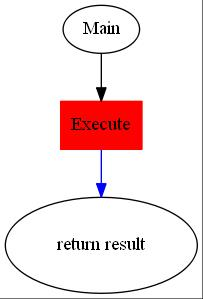
\includegraphics[scale=0.9]{Gambar/Graphviz.jpg}
\caption[Hasil output Graphviz]{Hasil output Graphviz} 
\label{fig:outGraphviz}
\end{figure}












